\documentclass[11pt]{article}

% package to include images
\usepackage{graphicx}

% parameters for \maketitle
\title{Computational Vision Lab 01}
\author{Johannes Heidecke}

% paragraph formatting
\setlength{\parindent}{2em}
\setlength{\parskip}{2em}
\renewcommand{\baselinestretch}{1.1}

% prevent orphans and widows
\widowpenalty10000
\clubpenalty10000

\begin{document}

\maketitle


\section*{Exercise 1:}

The three gray scale images are created in Matlab as simple matrices containing zeros and ones. These matrices are then concatenated along the third dimension to form the three color channels of the RGB image. See figure \ref{fig:task1}.

\begin{figure}[!hbt]
  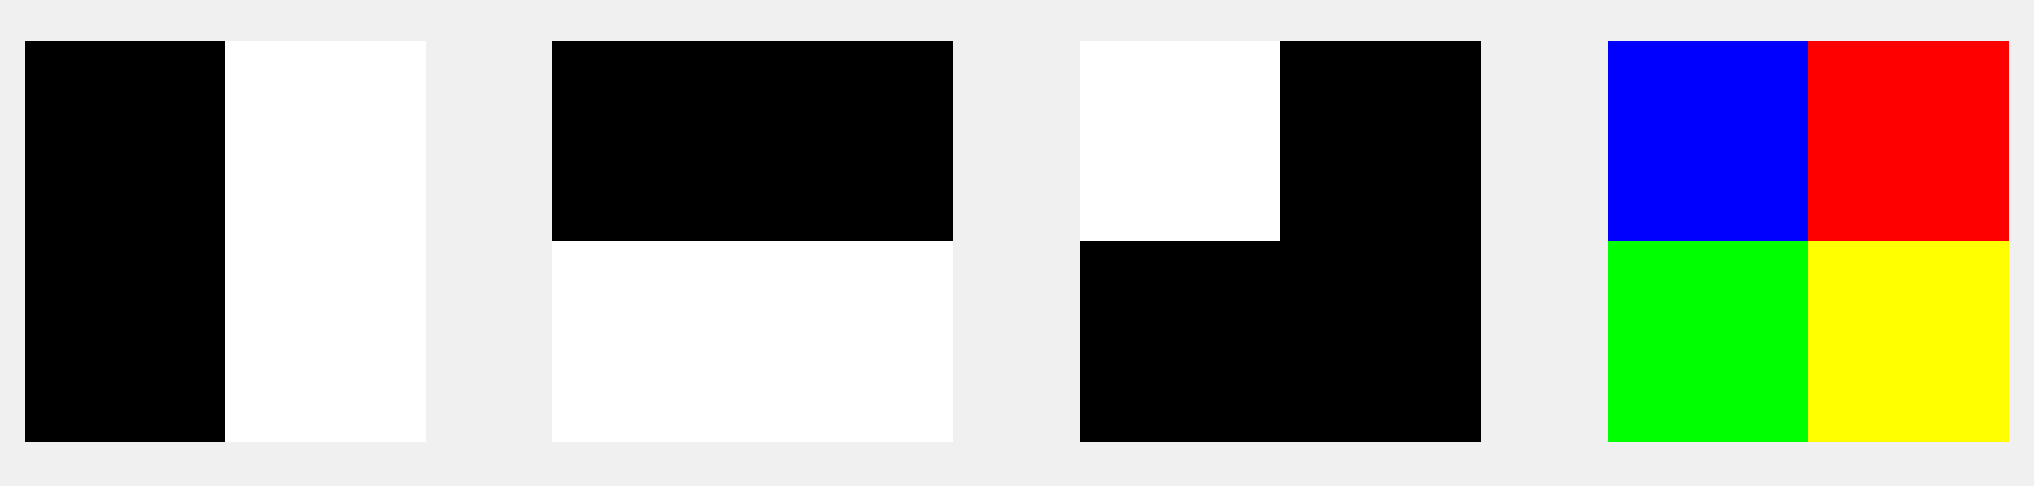
\includegraphics[width=\textwidth]{task1}
  \caption{Results of Exercise 1}
  \label{fig:task1}
\end{figure}


\section*{Exercise 2:}

The image \textit{chairs.jpg} consists of the three different color channels of the RGB spectrum: red, green and blue. Pixel that have a high portion of red color (e.g. the pillows on the chairs) have a very high value in the red color channel. Looking at the greyscale image of this channel, these pixels appear almost white. The very red pillows appear black in the green and blue channel, since their color does not contain a lot of green and blue. Colors that have a almost equal distribution of the three channels are perceived as the range from white, to gray, to black. The image contains mainly white and gray colors, for that reason the three channels look very much alike, as can be seen in figure \ref{fig:task2}.

\begin{figure}[!hbt]
  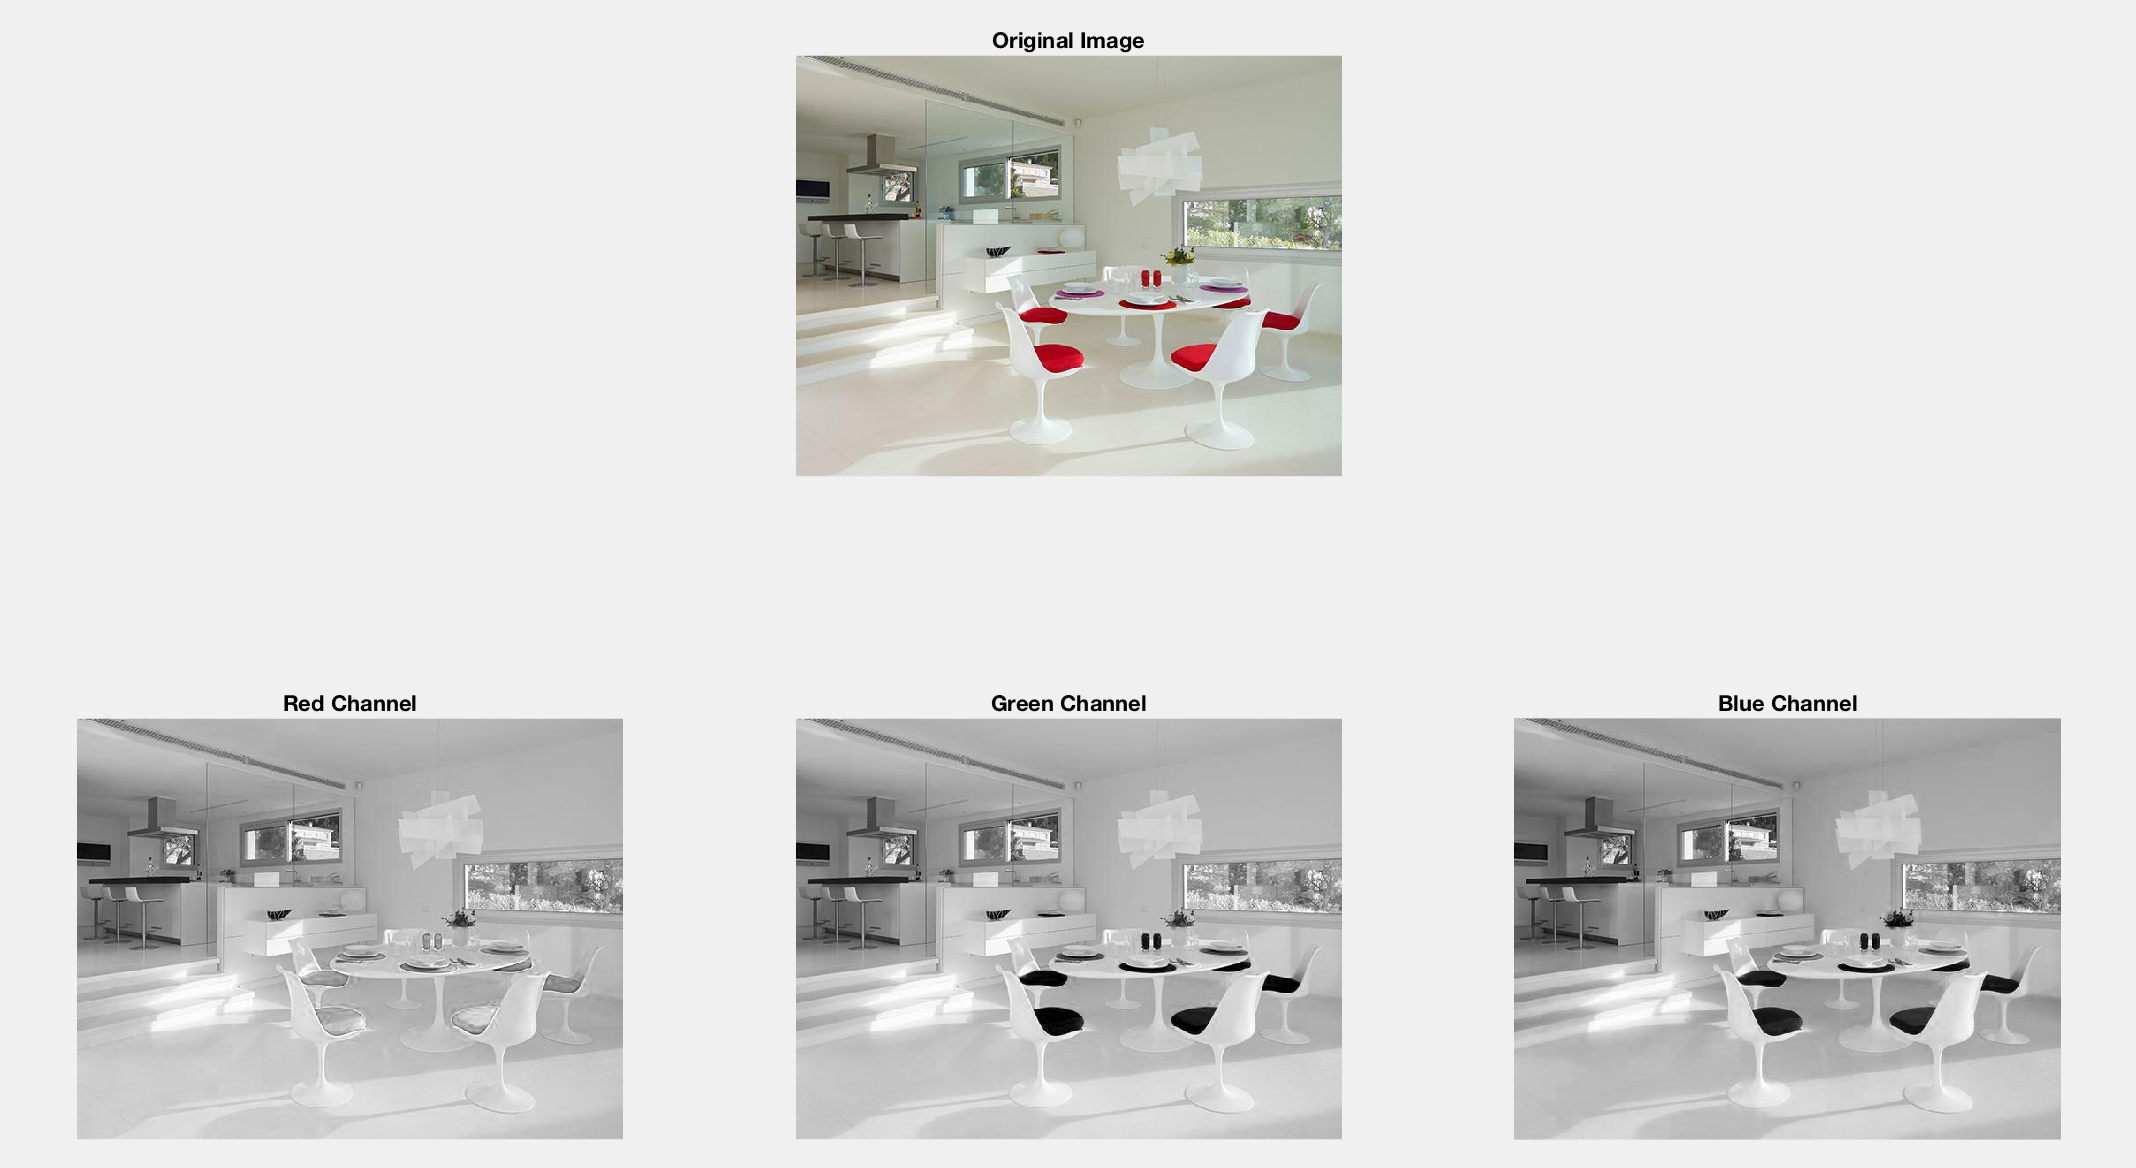
\includegraphics[width=\textwidth]{task2}
  \caption{Original Image and its three RGB channels}
  \label{fig:task2}
\end{figure}

It is possible to interchange the different channels with each other. Since there are three channels, 6 different permutations are possible, with one of them being the normal RGB order. The results of those permutations can be seen in figure \ref{fig:task3}.

\begin{figure}[!hbt]
  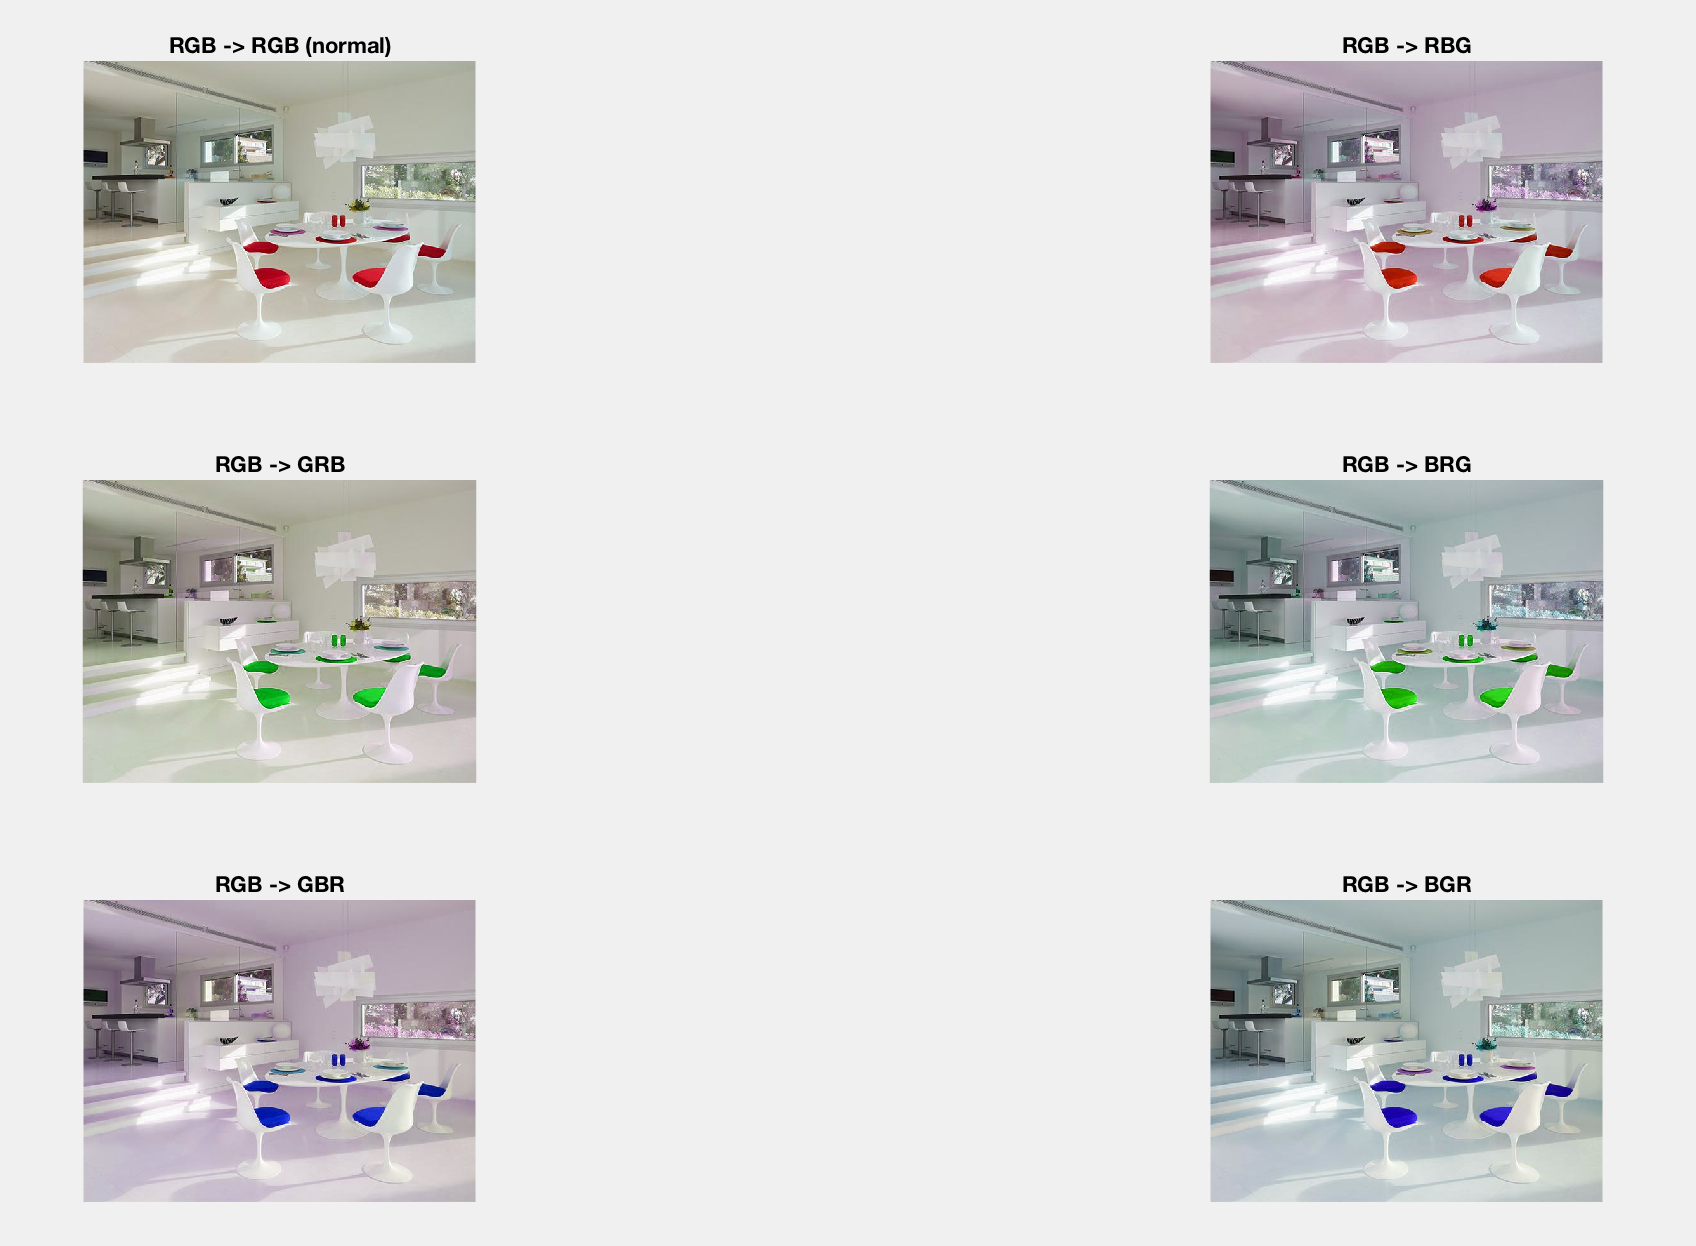
\includegraphics[width=\textwidth]{task3}
  \caption{Interchanging the RGB channels}
  \label{fig:task3}
\end{figure}

It is also possible to completely turn off single channels by multiplying all values of a channel by zero. The resulting images are colored in cyan, magenta, and yellow - exactly the colors that are being used in the subtractive color model of printing. The results are shown in figure \ref{fig:task4}.

\begin{figure}[!hbt]
  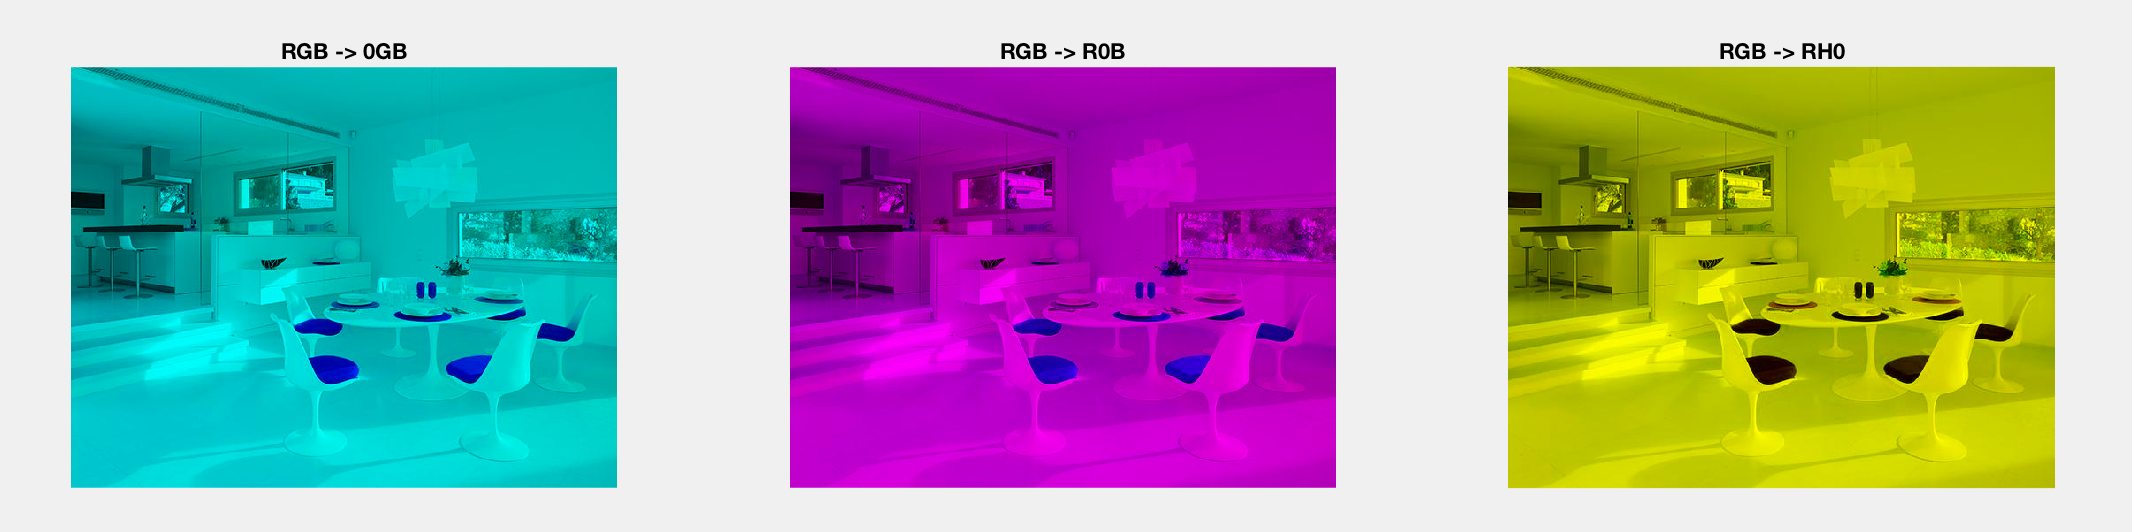
\includegraphics[width=\textwidth]{task4}
  \caption{Deactivating single RGB channels}
  \label{fig:task4}
\end{figure}

\section*{Exercise 3:}

Resizing an image to a smaller size reduces not only the size but also the details of the image. This can be seen in figure \ref{fig:task5}. While a rescaling to 0.5 times the original size still shows most of the details of this particular image, after rescaling it to 0.01 size almost all details are lost.

\begin{figure}[!hbt]
  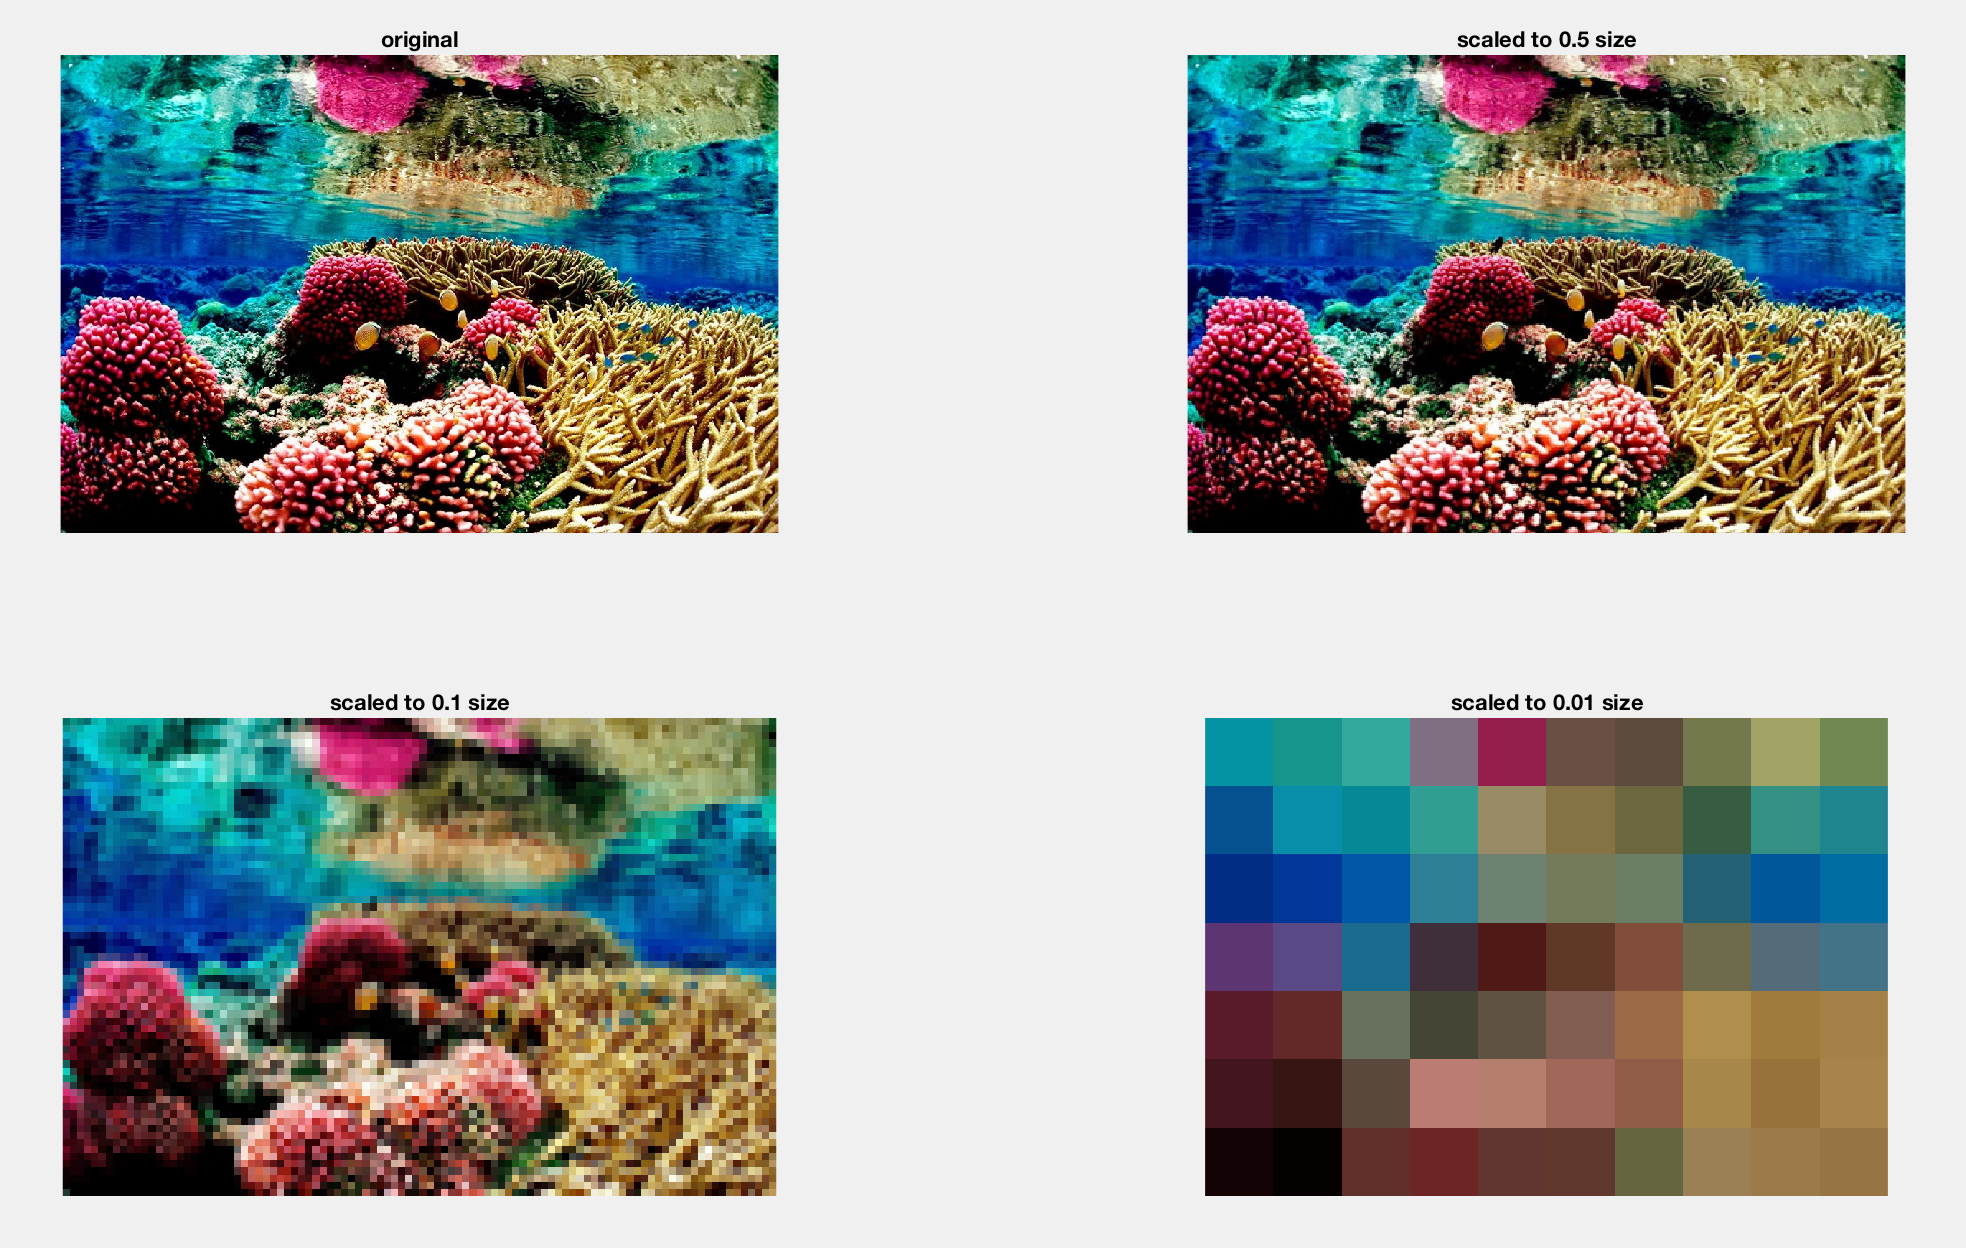
\includegraphics[width=\textwidth]{task5}
  \caption{Resizing the original image to smaller sizes}
  \label{fig:task5}
\end{figure}

This loss of details after resizing can also be observed in the histogram of the three color channels. 

\begin{figure}[!hbt]
  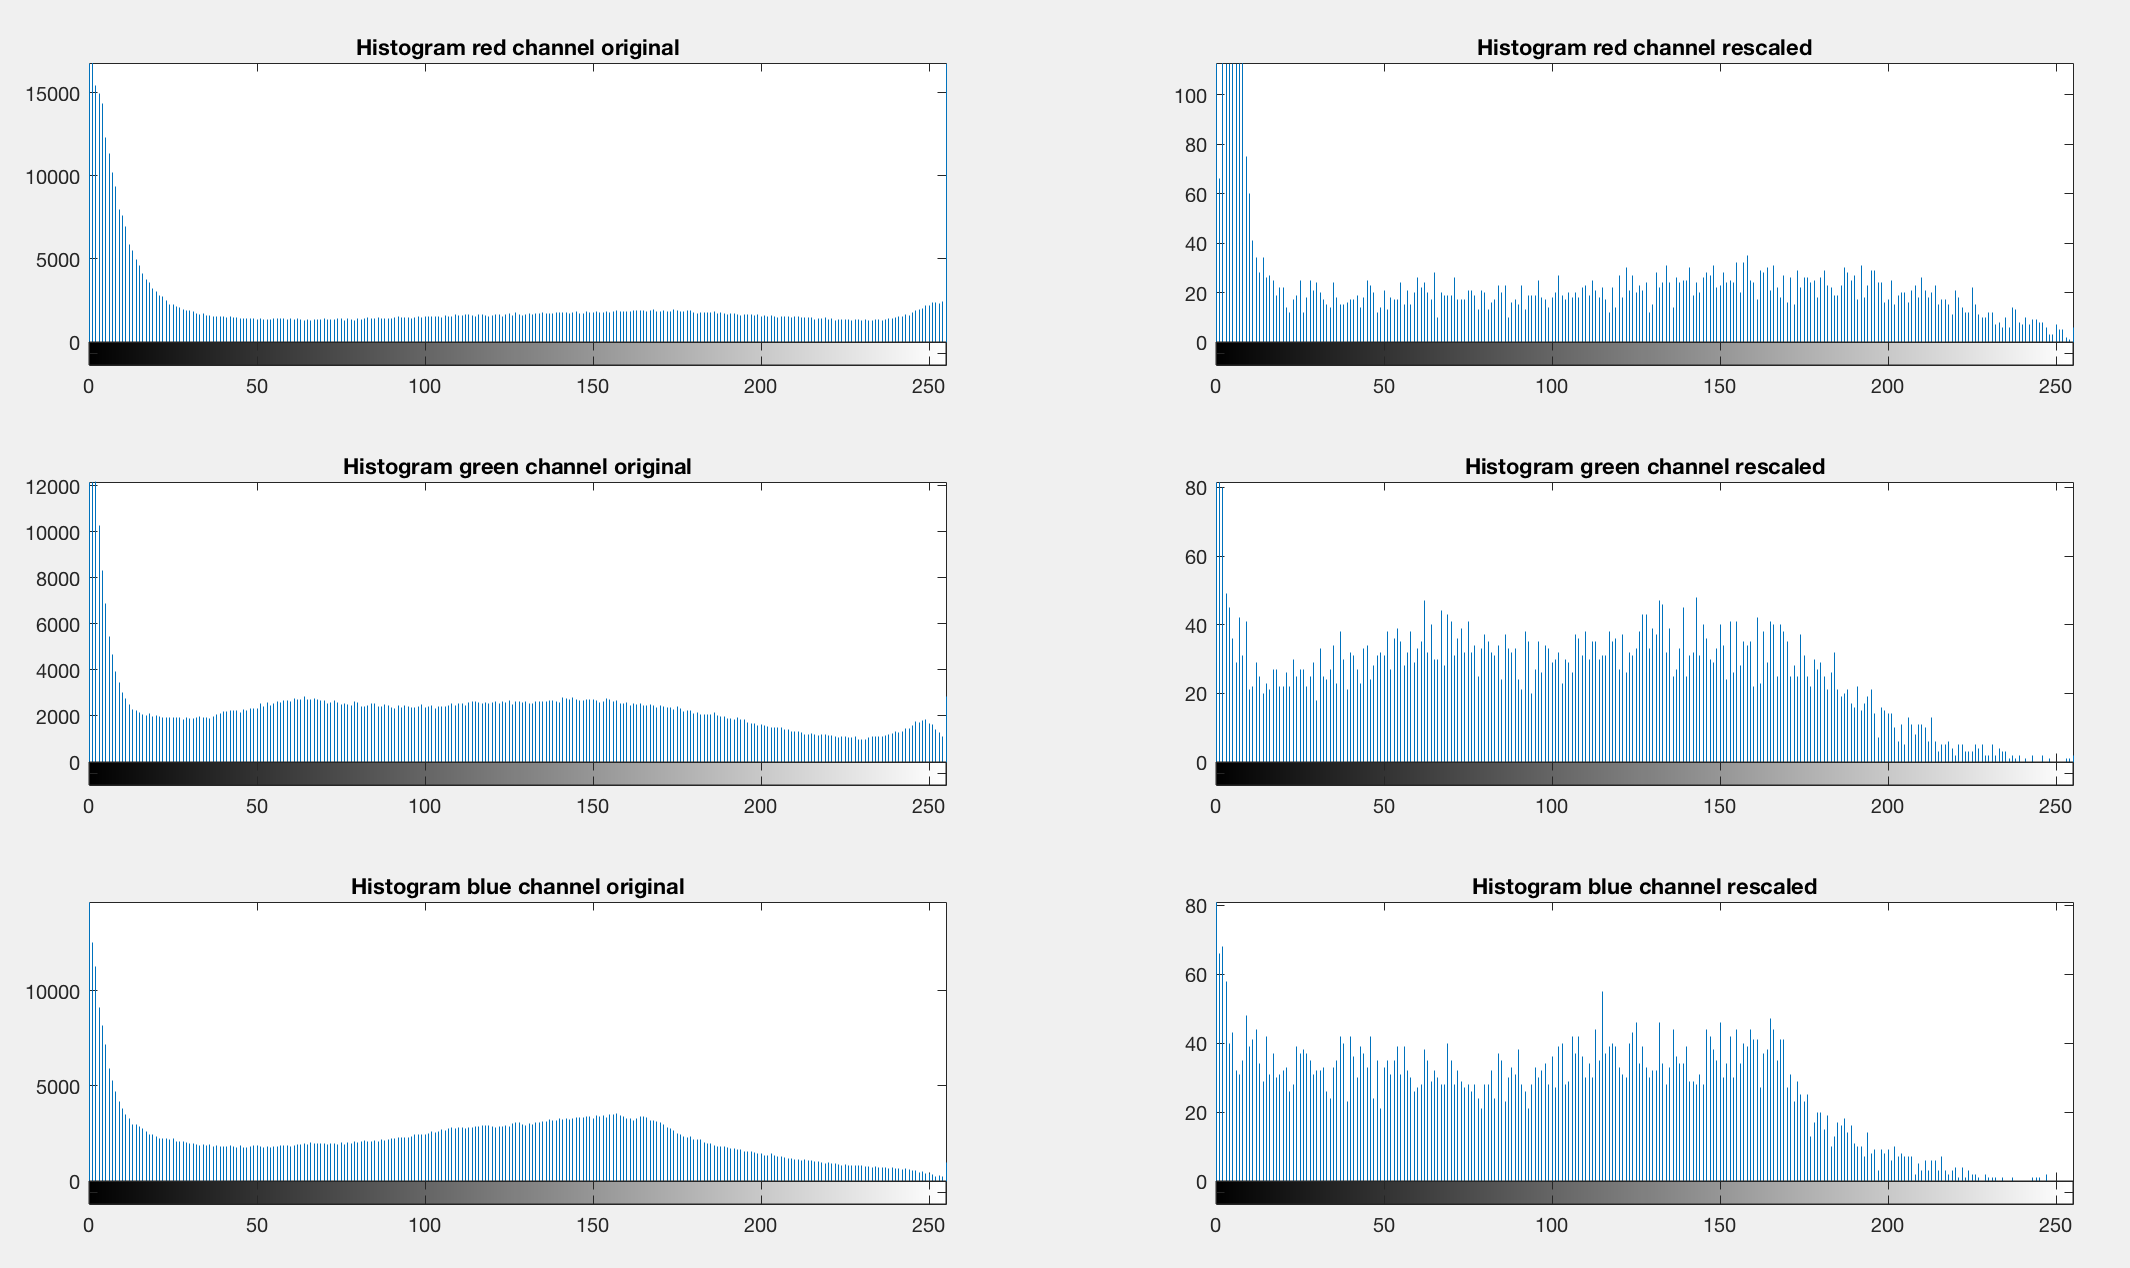
\includegraphics[width=\textwidth]{task6}
  \caption{Change of the RGB histograms after resizing to 0.1 original size}
  \label{fig:task6}
\end{figure}


\end{document}
